\documentclass[journal=jcisd8,manuscript=article]{achemso}

\usepackage[T1]{fontenc}
\usepackage{amsmath}
\usepackage{amssymb}
\usepackage{microtype}
\usepackage{graphicx}
\graphicspath{{figures/}}
\usepackage{booktabs}
\usepackage{siunitx}
\usepackage{xcolor}
\usepackage{hyperref}
\usepackage{xurl}
\usepackage{setspace}
\usepackage{placeins}
\usepackage{float}
\usepackage{caption}

\sisetup{
  separate-uncertainty=true,
  multi-part-units=single
}
\DeclareSIUnit\angstrom{\text{\AA}}

\hypersetup{hidelinks}

% Add more breathing room around floats (especially tables).
\setlength{\textfloatsep}{18pt}
\setlength{\intextsep}{16pt}
\setlength{\floatsep}{12pt}
\floatplacement{figure}{htbp}
\floatplacement{table}{htbp}
\renewcommand{\topfraction}{0.9}
\renewcommand{\bottomfraction}{0.9}
\renewcommand{\textfraction}{0.1}
\renewcommand{\floatpagefraction}{0.8}
\captionsetup[table]{skip=6pt}

\title{Boltz-2 Outperforms AutoDock Vina on Lipid--Protein Complex Prediction}

\author{Jackson Stempel}
\affiliation{Department of Biochemistry \& Cellular and Molecular Biology, University of Tennessee, Knoxville, Tennessee 37996, United States}

\author{Micholas Smith}
\email{msmit316@utk.edu}
\affiliation{Biosciences Division and Center for Molecular Biophysics, Oak Ridge National Laboratory, Oak Ridge, Tennessee 37831, United States}
\alsoaffiliation{Department of Biochemistry \& Cellular and Molecular Biology, University of Tennessee, Knoxville, Tennessee 37996, United States}

\abbreviations{PDB, Protein Data Bank; RMSD, root-mean-square deviation; MCS, maximum common substructure; MSA, multiple sequence alignment}
\keywords{lipid docking, docking benchmarks, membrane proteins, Boltz-2, AutoDock Vina, GNINA}

\begin{document}

\pagestyle{plain}

\doublespacing

\begin{abstract}
Lipid--protein interactions are central to membrane biology, but lipid docking remains difficult because flexible hydrocarbon tails coexist with chemically specific headgroup contacts.
Here we benchmark Boltz-2 against AutoDock Vina on 100 curated lipid--protein complexes; Vina and GNINA are evaluated in a binding-site-known re-docking setting, whereas Boltz-2 is evaluated as blind sequence-and-ligand complex prediction.
We score predictions with complementary geometric metrics (ligand and headgroup RMSD) and interaction-based metrics (headgroup contact overlap).
Boltz-2 substantially outperforms Vina, achieving a median ligand RMSD of \SI{1.26}{\angstrom} versus \SI{4.37}{\angstrom} for Vina top-1 ($p = 2.2 \times 10^{-12}$, Wilcoxon signed-rank test), with 73\% (95\% CI 64--81) versus 12\% (95\% CI 7--20) of predictions within \SI{2}{\angstrom}.
Boltz-2 also better recapitulates native protein--headgroup contacts (mean environment Jaccard 0.70 vs 0.39), while GNINA improves Vina's top-1 ranking but remains below Boltz-2.
To test whether Boltz-2 reflects learned interaction physics rather than positional memorization, we performed an adversarial mutagenesis experiment in which binding-site residues were mutated to glycine or phenylalanine and predictions were rerun.
Among initially accurate wild-type cases, only 23\% (Gly) and 20\% (Phe) remained below \SI{3}{\angstrom} after mutation, indicating that Boltz-2's lipid placement depends on local binding-site chemistry rather than simple memorization.
\end{abstract}

\section{Introduction}

Lipids are essential biomolecules that function as membrane components, signaling molecules, and energy stores.\cite{vanmeer2008membrane}
Understanding lipid--protein interactions is therefore central to membrane protein function, lipid transport, and disease mechanisms involving lipid dysregulation.\cite{escriba2008membranes}
Despite advances in structural biology, experimentally determining lipid binding poses and assigning functionally relevant bound lipids remain difficult, motivating computational docking methods.\cite{hunte2008lipids}

Molecular docking is a standard tool for predicting protein--ligand binding modes.\cite{kitchen2004docking}
Physics-based methods such as AutoDock Vina use empirical scoring functions to rank candidate poses,\cite{trott2010autodock} and CNN-based rescoring methods such as GNINA aim to improve ranking without changing the underlying sampling procedure.\cite{mcnutt2025gnina13}
Deep learning has since transformed biomolecular structure prediction: AlphaFold2 revolutionized protein structure prediction,\cite{jumper2021highly} and later models including AlphaFold3 extended this capability to protein--ligand complexes.\cite{abramson2024accurate}
Boltz-2 is an open-source diffusion-based model for biomolecular complex prediction that jointly models protein and ligand conformations.\cite{passaro2025boltz2,wohlwend2024boltz}

Lipids present challenges that differ from those of typical drug-like ligands.
Their hydrocarbon tails are highly flexible, while the biologically relevant determinants of binding are often concentrated in the polar headgroup, which forms specific hydrogen-bonding and electrostatic contacts as the tail contributes largely hydrophobic packing.
In addition, many lipid binding sites lie at membrane interfaces or within transmembrane regions rather than in conventional soluble-protein pockets.

Previous docking benchmarks have focused predominantly on drug-like molecules,\cite{wang2016comprehensive,su2019comparative} leaving lipid--protein docking relatively underexplored.
The limited lipid-docking literature emphasizes the difficulty of accurately predicting tail conformations and the importance of headgroup placement for biological relevance.\cite{sridhar2017computational}

Here we benchmark Boltz-2 against AutoDock Vina on 100 curated lipid--protein complexes; for the docking baselines (Vina and GNINA), each ligand is docked back into its cognate experimental receptor in a binding-site-known re-docking setting.
We evaluate predictions with both geometric metrics (ligand and headgroup RMSD) and interaction-based metrics (protein--headgroup contact overlap), and we discuss the distinction between re-docking and prospective prediction.
Our contributions are fourfold: (i) a curated lipid--protein docking benchmark with standardized evaluation across docking and structure-prediction methods, (ii) a metric suite that separates tail-dominated geometric error from headgroup placement and interaction fidelity, (iii) an analysis that disentangles sampling quality from ranking quality for classical docking baselines, and (iv) an adversarial mutagenesis experiment probing whether AI-based predictions reflect learned physical principles or memorization.

\begin{figure}[H]
\centering
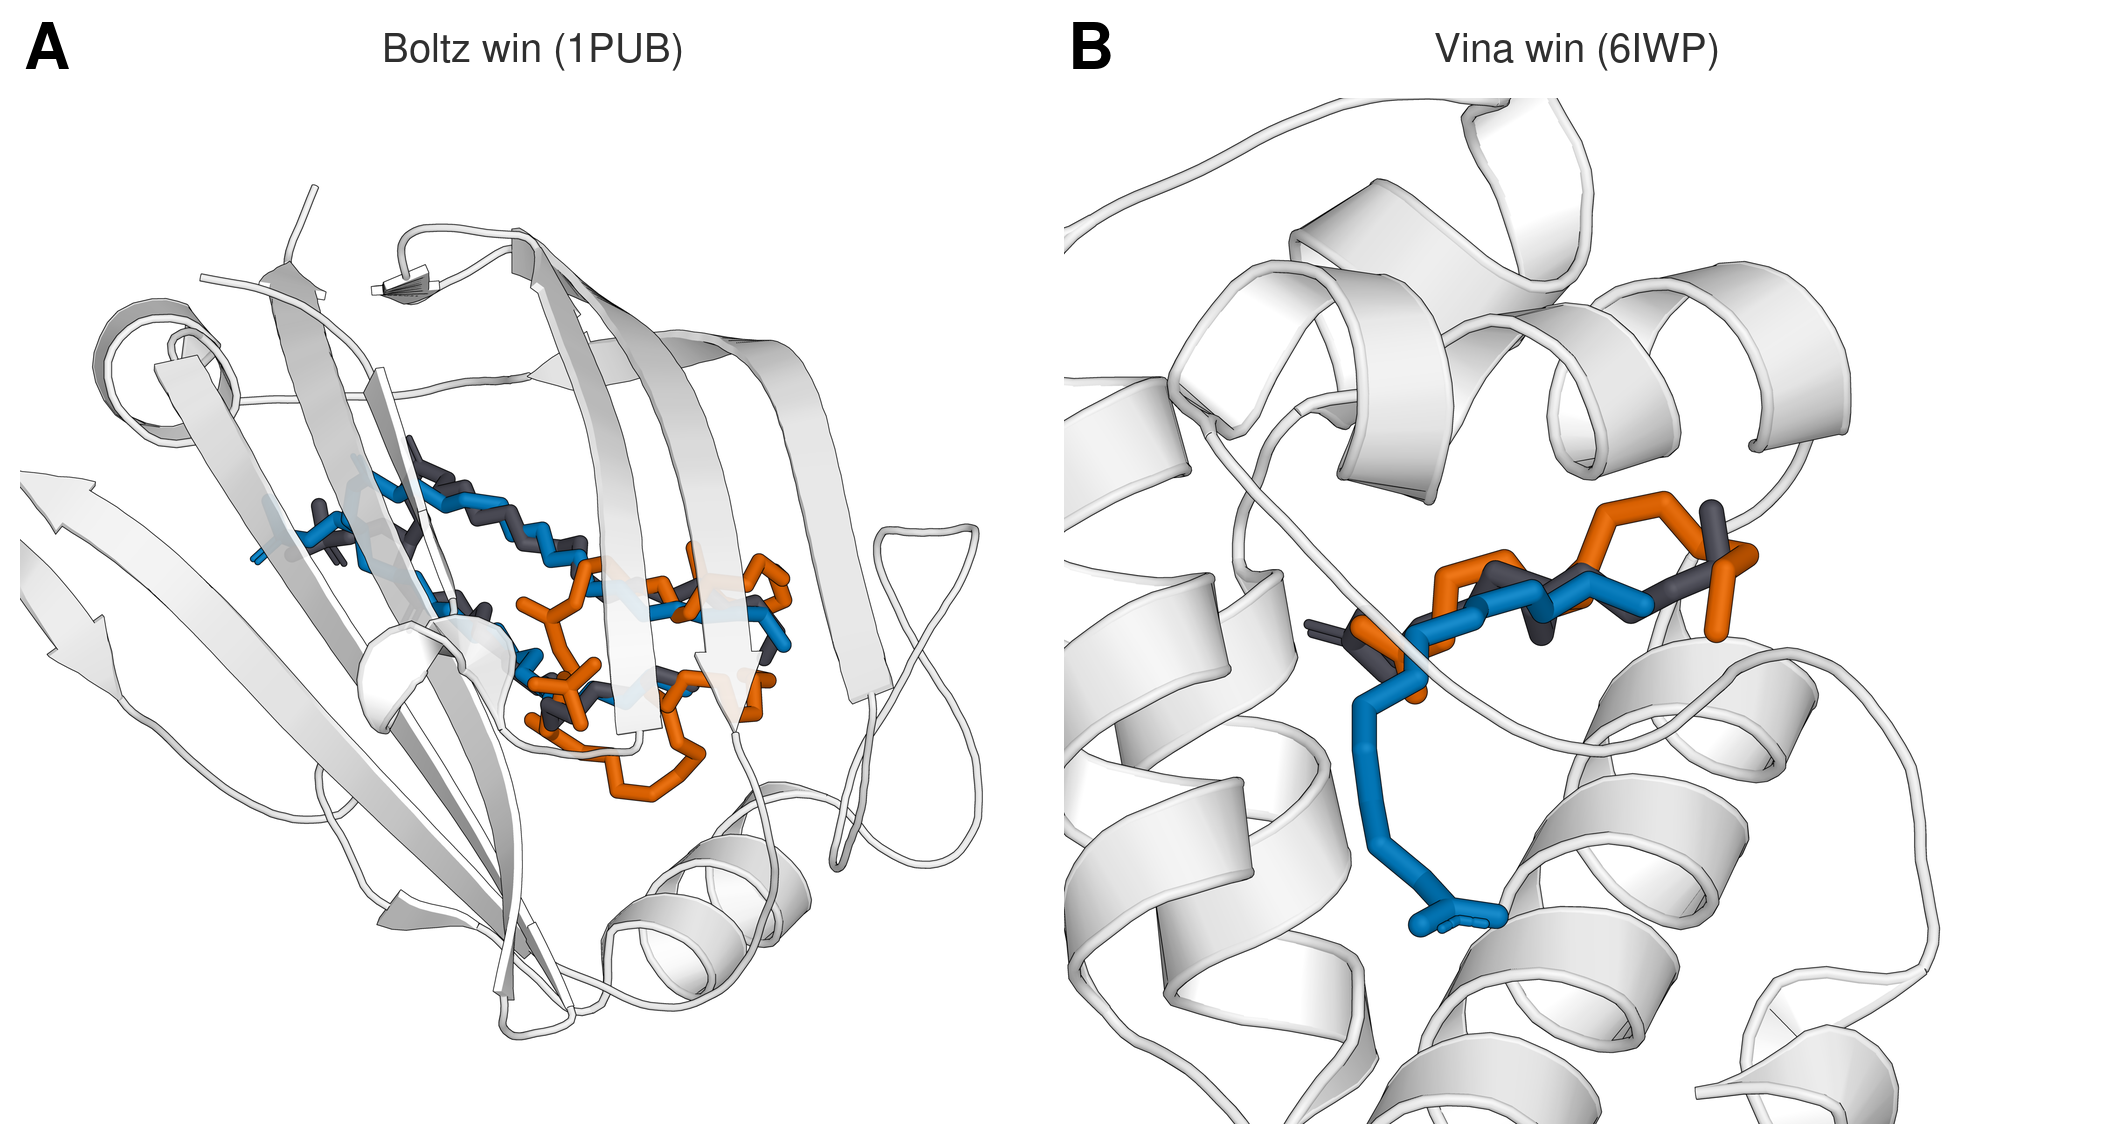
\includegraphics[width=\columnwidth]{fig_structural_examples.png}
\caption{Representative qualitative examples of lipid pose prediction outcomes. (A) For PDB 1PUB, Boltz-2 recovers the native 3PH pose (RMSD \SI{1.58}{\angstrom}), whereas Vina top-1 collapses the same high-degree-of-freedom lipid into a jumbled non-native conformation (RMSD \SI{10.64}{\angstrom}). (B) For PDB 6IWP, Vina top-1 recovers a near-native MYR pose (RMSD \SI{2.67}{\angstrom}) while Boltz-2 fails (RMSD \SI{11.07}{\angstrom}). Experimental ligands are shown in dark gray, Boltz-2 predictions in blue, and Vina top-1 poses in orange; proteins are shown as light-gray cartoons.}
\label{fig:structural_examples}
\end{figure}

\section{Methods}

\subsection{Benchmark Dataset Curation}

We assembled a benchmark set of lipid--protein complexes from the Protein Data Bank (PDB).\cite{berman2000protein}
For this study, we define lipids as amphipathic molecules containing both a polar headgroup and one or more hydrocarbon chains, including fatty acids, phospholipids, glycolipids, and sterols.

Starting from PDB structures containing bound lipid ligands, we applied the following curation criteria to ensure unambiguous evaluation:

\begin{enumerate}
    \item \textbf{Single ligand requirement}: Structures with multiple lipid ligands or ambiguous ligand identity were excluded to enable unambiguous atom-wise comparison between predicted and experimental poses.
    \item \textbf{Single protein chain}: We restricted the benchmark to single-chain protein complexes to simplify alignment.
    \item \textbf{Chemistry validation}: Ligands were validated using RDKit\cite{rdkit} to ensure correct valence states and recognized elements; structures with chemistry errors were excluded.
    \item \textbf{Atom mapping coverage (evaluation)}: RMSD calculations required RDKit MCS atom correspondences. Predicted poses were considered valid if $\geq$90\% of predicted heavy atoms matched the reference and $\geq$60\% of reference heavy atoms were covered; partial matches (reference coverage $<$90\%) were flagged explicitly.
\end{enumerate}

In total, we considered 159 candidate complexes and excluded 58 entries during curation due to RDKit failures, insufficient atom-mapping coverage, or file parsing issues.

After curation, we excluded one outlier target (PDB 3L1N) due to severe protein RMSD in Boltz-2 predictions, leaving 100 complexes for all analyses reported here.
The dataset spans diverse lipid types including fatty acids (e.g., palmitate, oleate), phospholipids (e.g., phosphatidylcholine derivatives), glycolipids (e.g., GM3), and sterols (e.g., cholesterol), with ligand sizes ranging from 11 to 102 heavy atoms (mean: 25.2 atoms).

\subsection{Docking Methods}

\subsubsection{Boltz-2}

Boltz-2 is an open-source biomolecular structure prediction model based on a diffusion architecture.\cite{passaro2025boltz2,wohlwend2024boltz}
Unlike docking, it predicts protein structure from sequence while jointly modeling the bound ligand conformation.
For each target, Boltz-2 was provided the protein sequence and ligand identity.
MSAs were generated automatically via the mmseqs2 server (accessed January 2026).\cite{mirdita2022colabfold}
We used \texttt{boltz predict} with MSA-server mode enabled and sampling settings of 200 diffusion steps, 3 recycling steps, and 1 diffusion sample (output format: mmCIF; other parameters at defaults).
We did not provide structural templates, pocket/contact constraints, receptor coordinates, or inference-time potentials; Boltz-2 was therefore evaluated in a fully blind sequence-and-ligand setting.

\subsubsection{AutoDock Vina}

AutoDock Vina is a physics-based docking program that uses an empirical scoring function combining steric, hydrophobic, hydrogen bonding, and torsional terms.\cite{trott2010autodock}
Unlike Boltz-2, Vina docks ligands into a rigid protein receptor.

For each target, we extracted the ligand from the experimental structure and docked it back into the corresponding experimental receptor after removing the ligand and crystallographic waters (ions retained); receptor and ligand preparation assumed pH 7.4 and used the PDBQT format required by Vina.
For reproducibility, the archived inputs for each target comprise a protein-only receptor structure (\path{receptor\_no\_ligand.pdb}), receptor and ligand PDBQT files (\path{receptor.pdbqt}, \path{ligand.pdbqt}), and a one-line search-box specification file.
The search box was centered on the experimental ligand centroid, and each dimension was set to the ligand's Cartesian extent plus a 6~\AA\ margin.
Vina was run with exhaustiveness 8 and configured to output up to 20 poses ranked by predicted binding affinity (estimated free energy of binding in kcal/mol).
All Vina runs used a fixed random seed (0) for reproducibility.
To investigate sensitivity to search effort, we also analyzed a full-dataset Vina rerun at exhaustiveness 256.

This setup is intentionally favorable to the docking baselines: the search box is derived from the experimental ligand position, giving Vina and GNINA a binding-site-known re-docking scenario.

\subsubsection{GNINA (Vina with CNN rescoring)}

GNINA is derived from Vina/smina and augments classical scoring with a convolutional neural network (CNN) that can rescore or rerank sampled poses.\cite{mcnutt2025gnina13}
It therefore provides an intermediate baseline that retains Vina-like sampling while adding a learned scoring component.

In our ISAAC workflow, GNINA used the same target-specific search boxes as Vina, along with the archived protein-only receptor PDB and prepared ligand PDBQT inputs.
We also ran GNINA with CNN rescoring disabled (\path{cnn_scoring=none}) to isolate the effect of the CNN on ranking.
For any multi-pose docking method (Vina or GNINA), we distinguish:
(i) \textbf{top-1} performance (the program's highest-ranked pose; the practically relevant case) from
(ii) \textbf{top-$K$ best} performance (the best RMSD among the top $K$ poses; an oracle upper bound that measures whether accurate poses exist somewhere in the candidate set, independent of ranking).
We therefore analyze both and additionally quantify the \emph{ranking gap} (top-1 RMSD minus top-20 best RMSD) as a direct measure of ranking quality.
Immediately before GNINA execution, the prepared ligand PDBQT was converted to SDF with OpenBabel inside the container to preserve explicit bonding, while outputs were written back to PDBQT for compatibility with the benchmark pipeline.

\subsubsection{Software and Versions}

AutoDock Vina runs used AutoDock Vina 23d1252-mod.
GNINA runs used GNINA 1.3.1 (Apptainer image, \path{gnina/gnina:latest}), with CNN rescoring enabled (\path{cnn_scoring=rescore}) unless otherwise specified.\cite{mcnutt2025gnina13}
Boltz runs used boltz 2.2.0.
\begin{sloppypar}
Benchmark evaluation used Python 3.12.11 with RDKit 2025.03.3, Biopython 1.84, Gemmi 0.7.3, NumPy 1.26.4, SciPy 1.13.1, PyYAML 6.0.2, pandas 2.3.1, PandaMap 4.1.0, matplotlib 3.10.7, SciencePlots 2.2.0, and cmocean 4.0.3.
\end{sloppypar}
ChimeraX was used for visual spot-checking of representative protein alignments, ligand placements, headgroup atom selections, and contact environments, including selected outlier cases.\cite{goddard2018chimerax}

\subsection{Structure Alignment}

To enable fair comparison, predicted complexes were aligned to experimental structures using the protein backbone.
Chain correspondence was determined by global sequence alignment with BioPython's PairwiseAligner,\cite{cock2009biopython} and corresponding C$\alpha$ atoms were fit using an iterative outlier-pruned least-squares superposition (2.0~\AA\ cutoff; Kabsch algorithm).
The resulting transformation was applied to both protein and ligand coordinates in the predicted complex.
Vina poses were evaluated directly in the experimental receptor coordinate frame and therefore did not require additional protein alignment.

\subsection{Geometric Metrics}

\subsubsection{Ligand RMSD}

Ligand RMSD was calculated over paired heavy atoms after placing predictions in the experimental reference frame (protein-backbone alignment for Boltz-2; direct evaluation in the experimental receptor frame for Vina).
Atom correspondence between predicted and experimental ligands was established using RDKit's maximum common substructure (MCS) mapping, and RMSD was computed over the paired atoms without an additional ligand-only fit.
As a robustness check for symmetric substructures, we performed a symmetry-aware mapping check and found no cases where the optimal correspondence changed (0/100 targets).
Predicted poses were considered valid if the MCS covered $\geq$90\% of predicted heavy atoms and $\geq$60\% of reference heavy atoms; cases with lower reference coverage were flagged as partial matches.
These thresholds were chosen to balance stringency against dataset retention, ensuring reliable mappings without discarding a large fraction of targets.

\subsubsection{Headgroup RMSD}

Because headgroup positioning is often the biologically relevant part of lipid binding, we also computed an RMSD restricted to headgroup atoms.
Headgroup atoms were identified automatically with a functional-group heuristic:
\begin{enumerate}
    \item If phosphorus atoms are present, the headgroup comprises all atoms within two bonds of any phosphorus.
    \item Otherwise, if nitrogen atoms with degree $\geq$3 exist, atoms within two bonds of such nitrogens define the headgroup.
    \item Otherwise, if any carbon has $\geq$2 oxygen neighbors, that carbon and its oxygen neighbors constitute the headgroup.
    \item Otherwise, all heteroatoms (O, N, P, S) are considered headgroup atoms.
\end{enumerate}
This rule set is intended to capture the polar functional groups that define lipid identity across chemically diverse ligands while remaining fully automated and reproducible.
Headgroup RMSD was computed over the mapped headgroup atom pairs.
Across the 100 targets, the headgroup selection contained a median of 3 atoms (IQR 2; range 1--19). A small number of sterol-like ligands have only a single polar atom, for which headgroup RMSD primarily reflects hydroxyl placement.
The headgroup definition rule was triggered by phosphorus atoms in 20 ligands, a cationic nitrogen criterion in 1, a carbonyl/oxygen-neighborhood criterion in 73, and by the final heteroatom rule in 7.

\subsection{Interaction Metrics}

Beyond geometric accuracy, we evaluated how well predictions recapitulate native protein--lipid interactions.

\subsubsection{Headgroup Environment Overlap}

We identified all protein residues with any heavy atom within \SI{5.0}{\angstrom} of any headgroup atom in both experimental and predicted structures.
This coarse, distance-based metric complements RMSD by evaluating whether the predicted headgroup occupies the correct residue environment even when specific interaction geometries are sparse or ambiguous.
The overlap between these residue sets was quantified using the Jaccard similarity coefficient:
\begin{equation}
    J = \frac{|R_\text{ref} \cap R_\text{pred}|}{|R_\text{ref} \cup R_\text{pred}|}
\end{equation}
where $R_\text{ref}$ and $R_\text{pred}$ are the sets of contacting residues in the reference and predicted structures, respectively.

\subsubsection{Typed Interaction Overlap}

We analyzed specific interaction types using PandaMap,\cite{pandamap} which detects hydrogen bonds, ionic interactions, salt bridges, and attractive charge interactions.
To focus on biologically informative features for lipids, we report Jaccard similarity over typed headgroup--protein interaction pairs.

\subsection{Multi-Pose Analysis}

For Vina, we report both the top-ranked pose (top-1) and ``top-$K$ best'' performance, where top-$K$ best denotes oracle selection of the lowest ligand RMSD among the first $K$ ranked poses ($K \in \{1,5,20\}$).
This analysis distinguishes intrinsic sampling capability from ranking accuracy.

\subsection{Statistical Analysis}

All method comparisons were performed on the same 100 targets.
Our primary hypothesis test compares Boltz-2 versus Vina top-1 ligand RMSD using a paired Wilcoxon signed-rank test with $\alpha = 0.05$.
Other method comparisons are reported descriptively.

\subsection{Adversarial Binding-Site Mutagenesis}

A key concern with AI-based structure prediction is whether models learn transferable physical principles or instead reproduce ligand placements memorized from training structures.\cite{masters2025physics}
To probe this for lipid--protein complexes, we designed an adversarial mutagenesis experiment inspired by recent binding-site mutation challenges for protein--ligand co-folding models.\cite{masters2025physics}

For each target, we defined binding-site residues as those with side-chain heavy atoms within \SI{5.0}{\angstrom} of any experimental headgroup heavy atom and then generated two mutant sequences:
\begin{enumerate}
    \item \textbf{Glycine sweep}: all binding-site residues mutated to glycine, removing side-chain chemistry while preserving backbone geometry.
    \item \textbf{Phenylalanine sweep}: all binding-site residues mutated to phenylalanine, introducing bulky hydrophobic groups that sterically occlude the binding site.
\end{enumerate}

Mutant sequences were run through Boltz-2 with the same ligand definitions and inference settings as the baseline predictions.
Predictions were evaluated with the same benchmark pipeline, using a protein-fold filter (protein RMSD $\leq$ \SI{2.0}{\angstrom}) to ensure that observed ligand displacements reflect local binding-site effects rather than global refolding.
If Boltz-2 relies mainly on memorized placements, predictions should remain accurate despite binding-site disruption; if it relies on learned interactions, the mutations should displace the headgroup substantially.

\section{Results}

\subsection{Overall Docking Accuracy}

Boltz-2 substantially outperformed AutoDock Vina across all geometric metrics (Table~\ref{tab:summary}, Figure~\ref{fig:top1_rmsd}).
For ligand RMSD, Boltz-2 achieved a mean of \SI{2.20}{\angstrom} (median \SI{1.26}{\angstrom}) versus \SI{5.11}{\angstrom} (median \SI{4.37}{\angstrom}) for Vina top-1.
GNINA with CNN rescoring improved top-1 ligand RMSD (mean \SI{3.46}{\angstrom}, median \SI{2.31}{\angstrom}) relative to Vina, while GNINA without CNN rescoring was intermediate (mean \SI{4.57}{\angstrom}, median \SI{3.47}{\angstrom}).
This difference was highly significant for Boltz-2 versus Vina top-1 ($p = 2.2 \times 10^{-12}$, Wilcoxon signed-rank test).
Boltz-2 predictions cluster near the experimental structure, with 73\% within \SI{2}{\angstrom}, whereas only 12\% of Vina top-1 poses reached sub-\SI{2}{\angstrom} accuracy; GNINA-CNN improves this to 44\%.
The corresponding Wilson 95\% confidence intervals are 73\% [64--81] for Boltz-2 and 12\% [7--20] for Vina top-1.

		\FloatBarrier
		\begin{table}[H]
		\centering
		\scriptsize
		\setlength{\tabcolsep}{2pt}
		\caption{Summary of docking performance on 100 lipid--protein complexes. Values shown are mean (median) [IQR]. ``Vina top-K best'' denotes oracle selection of the lowest ligand RMSD among the first $K$ ranked poses (with all other metrics reported for that same pose). Typed interaction overlap is computed over targets with non-empty reference headgroup interactions (83/100).}
		\label{tab:summary}
	\begin{tabular}{@{}lcccc@{}}
\toprule
 & Ligand RMSD (\AA) & Headgroup RMSD (\AA) & Env.\ Jaccard & Typed Jaccard \\
\midrule
Boltz-2 & 2.20 (1.26) [1.22] & 2.38 (1.76) [1.50] & 0.70 (0.76) [0.28] & 0.69 (0.80) [0.52] \\
Vina top-1 & 5.11 (4.37) [4.18] & 5.52 (4.42) [5.54] & 0.39 (0.40) [0.60] & 0.34 (0.25) [0.67] \\
GNINA CNN top-1 & 3.46 (2.31) [2.75] & 3.16 (2.15) [2.14] & 0.62 (0.70) [0.39] & 0.57 (0.60) [0.80] \\
GNINA no-CNN top-1 & 4.57 (3.47) [3.97] & 5.05 (3.73) [5.46] & 0.44 (0.48) [0.62] & 0.36 (0.25) [0.67] \\
Vina top-20 best & 2.55 (1.77) [1.13] & 2.79 (2.02) [1.20] & 0.63 (0.67) [0.34] & 0.57 (0.50) [0.67] \\
\bottomrule
	\end{tabular}
	\end{table}

Vina top-20 best achieves substantially lower ligand RMSD than Vina top-1 and improves contact overlap, but it still trails Boltz-2 across metrics.
Headgroup RMSD followed the same trend, indicating that Boltz-2 improves not only whole-ligand placement but also the positioning of the functionally critical headgroup.

\FloatBarrier
\begin{figure}[H]
\centering
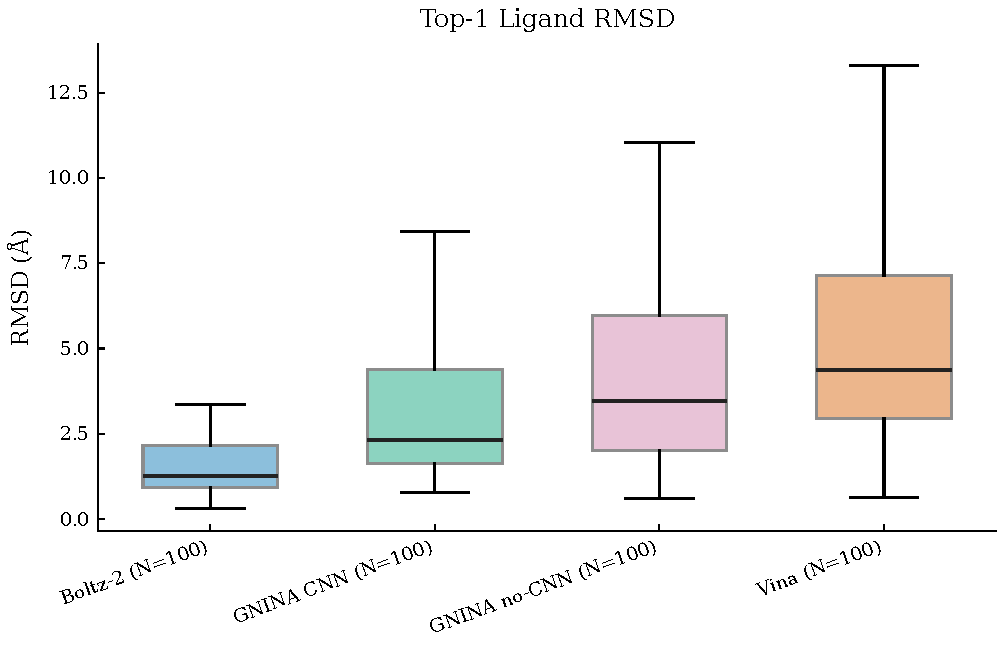
\includegraphics[width=0.9\columnwidth]{fig_top1_rmsd_methods.pdf}
\caption{Top-1 ligand RMSD distributions across methods. GNINA-CNN improves Vina accuracy but does not reach Boltz-2 performance.}
\label{fig:top1_rmsd}
\end{figure}

\subsection{Per-Target Comparison}

Pairwise comparison across all 100 targets reveals that Boltz-2 outperforms Vina on the large majority of complexes (Figure~\ref{fig:paired}).
Boltz-2 achieved lower ligand RMSD than Vina top-1 in 83 of 100 cases (83\%).
Even when comparing against Vina's oracle-selected best pose among 20 candidates, Boltz-2 remained superior in 65 cases (65\%).
GNINA-CNN outperformed Vina top-1 in 71 of 100 cases, reflecting a consistent (but smaller) improvement in ranking quality.

\begin{figure}[!t]
\centering
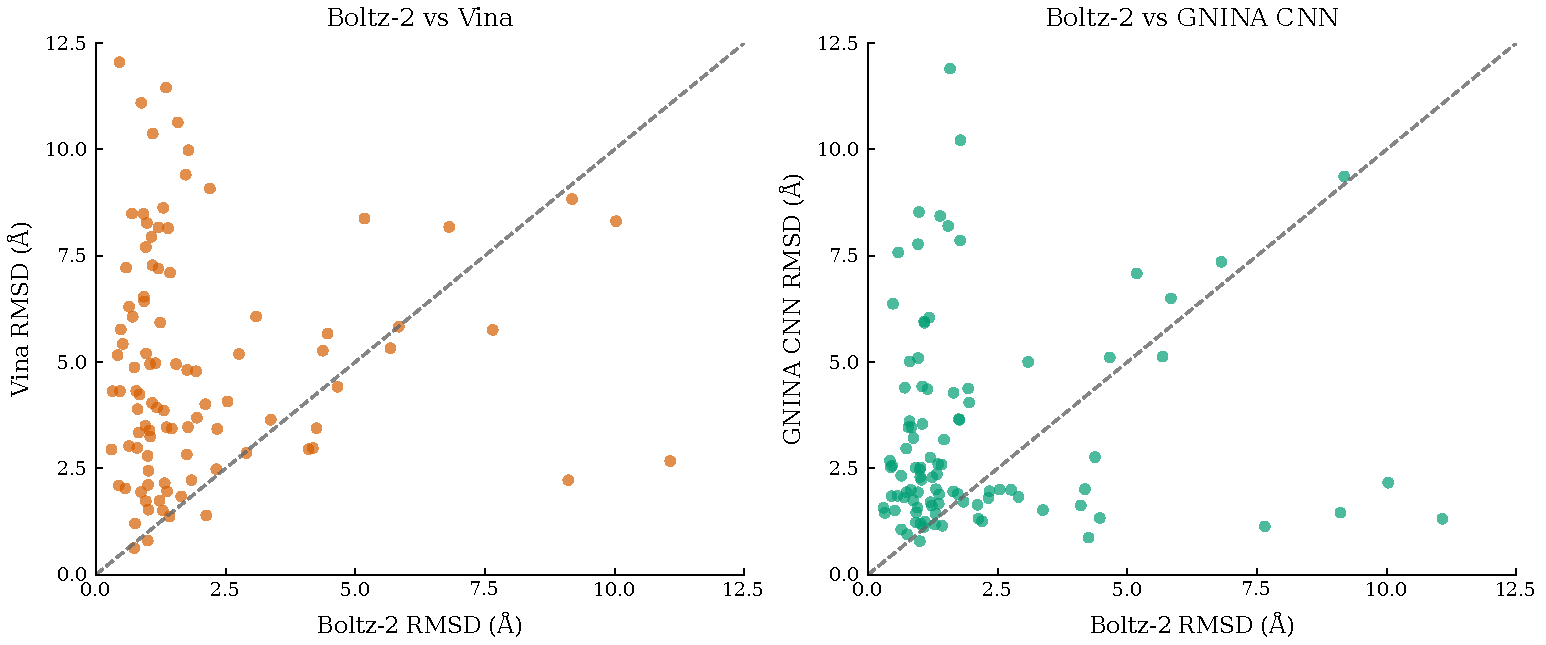
\includegraphics[width=\columnwidth]{fig_per_target_comparison_gnina.pdf}
\caption{Per-target ligand RMSD comparisons. Left: Boltz-2 vs Vina. Right: Boltz-2 vs GNINA-CNN. Points above the diagonal favor Boltz-2.}
\label{fig:paired}
\end{figure}
\FloatBarrier

\subsection{Sampling vs Ranking: Vina and GNINA}

Vina's multi-pose output shows that accurate poses often exist among lower-ranked candidates.
Its best-of-20 ligand RMSD (mean \SI{2.55}{\angstrom}, median \SI{1.77}{\angstrom}) is far better than its top-1 RMSD (mean \SI{5.11}{\angstrom}), indicating that sampling is often adequate but ranking is weak.
This separation between sampling and ranking is consistent with broader docking benchmarks that distinguish docking power from scoring power,\cite{wang2016comprehensive,su2019comparative} and supplemental robustness checks did not alter the qualitative picture: a full-dataset Vina exhaustiveness-256 rerun left the top-1 versus top-20 story unchanged, and a higher-sampling Boltz-2 rerun on 99 shared targets produced only minor aggregate shifts (Table S2, Supporting Information).
Figure~\ref{fig:structural_examples} illustrates two qualitatively distinct Vina failure modes observed during case review: on highly flexible lipids it can collapse into a visibly tangled non-native pose (Panel A), and in other cases not shown here it can occupy the correct pocket but invert the ligand orientation, yielding deceptively plausible pocket-level overlap despite poor RMSD.

GNINA shifts the best-of-20 distribution toward lower RMSD relative to Vina, indicating modestly improved sampling (or local refinement) in addition to better ranking.
GNINA-CNN achieves a best-of-20 mean ligand RMSD of \SI{1.95}{\angstrom} (median \SI{1.51}{\angstrom}) and reduces the ranking gap (top-1 minus best-of-20) from \SI{2.56}{\angstrom} for Vina to \SI{1.51}{\angstrom} (Figure~\ref{fig:sampling_ranking}).
GNINA without CNN rescoring shows a gap similar to Vina (\SI{2.53}{\angstrom}), implying that the CNN primarily improves ranking rather than sampling.

\begin{figure}[htbp]
\centering
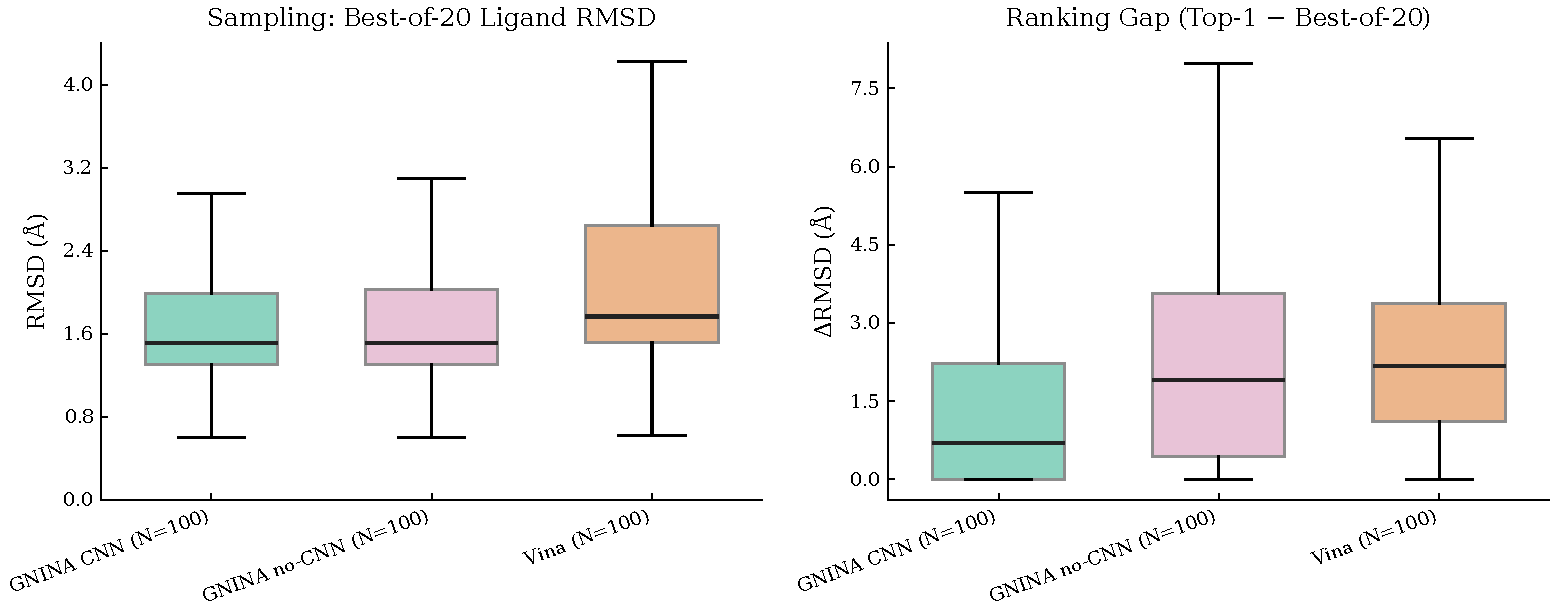
\includegraphics[width=0.95\columnwidth]{fig_sampling_vs_ranking.pdf}
\caption{Sampling vs ranking behavior for Vina and GNINA. Left: best-of-20 ligand RMSD distributions (sampling quality; Boltz-2 omitted because it produces a single pose). Right: ranking gap defined as top-1 minus best-of-20 ligand RMSD (positive values indicate ranking error). GNINA-CNN narrows the ranking gap relative to Vina.}
\label{fig:sampling_ranking}
\end{figure}
\FloatBarrier

\subsection{Interaction Fidelity}

Geometric accuracy translated into improved interaction recovery (Figure~\ref{fig:contacts_methods}).
Boltz-2 predictions achieved a mean headgroup environment Jaccard of 0.70 (median 0.76), whereas Vina top-1 reached 0.39 (median 0.40).
GNINA-CNN improved headgroup environment overlap to 0.62 (median 0.70), paralleling its improved headgroup RMSD.

Typed interaction analysis showed similar trends.
Boltz-2 achieved a mean typed interaction Jaccard of 0.69 (median 0.80), while Vina top-1 reached 0.34 (median 0.25); GNINA-CNN improved to 0.57 (median 0.60).
These results indicate that improved pose ranking yields more biologically relevant headgroup contacts.

\begin{figure}[htbp]
\centering
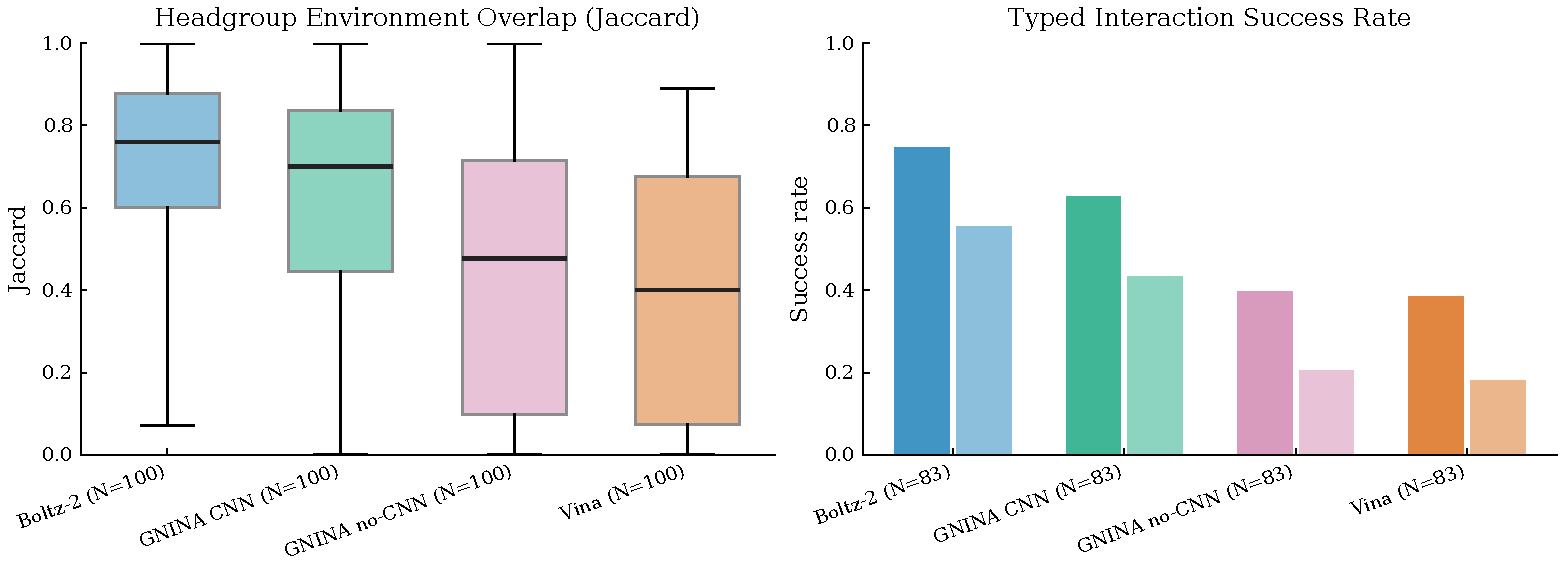
\includegraphics[width=0.95\columnwidth]{fig_contact_overlap_methods.pdf}
\caption{Headgroup interaction fidelity for top-1 poses. Left: headgroup environment overlap (Jaccard) shown as boxplots (median and interquartile range; whiskers indicate 5th--95th percentiles). Right: typed interaction success rate at Jaccard thresholds of 0.50 and 0.75. GNINA-CNN improves Vina's contact recovery but does not reach Boltz-2 performance.}
\label{fig:contacts_methods}
\end{figure}
\FloatBarrier

\subsection{Performance Stratified by Ligand Flexibility}

An exploratory stratification by ligand flexibility using Vina \texttt{TORSDOF} suggested that Boltz-2 remained relatively stable across bins, whereas Vina accuracy degraded with increasing torsion count even under oracle top-20 selection (Table S3, Supporting Information). The medium and high torsion bins were small ($n=13$ and $n=6$) and should therefore be interpreted descriptively.

Inspection of the 10 worst Boltz-2 predictions by ligand RMSD likewise suggested that most extreme failures involve severe headgroup misplacement and loss of contact overlap rather than tail-only deviations (Table S4, Supporting Information).

\subsection{Adversarial Mutagenesis: Probing Memorization vs.\ Physics}

To test whether Boltz-2's lipid placement reflects learned physical interactions or memorization, we evaluated predictions on binding-site mutants (Figure~\ref{fig:adversarial}).
Using a stricter fold-preservation cutoff (protein RMSD $\leq$ \SI{2.0}{\angstrom}), 89\% (Gly) and 91\% (Phe) of targets pass the fold filter, indicating that the observed ligand displacements largely reflect local binding-site perturbations rather than global refolding.

Wild-type Boltz-2 predictions achieved headgroup RMSD $<$ \SI{3}{\angstrom} in 88\% of targets (median \SI{1.76}{\angstrom}).
Upon glycine sweep, this dropped to 20\% (median \SI{5.14}{\angstrom}); upon phenylalanine sweep, to 18\% (median \SI{6.86}{\angstrom}).
The phenylalanine sweep produced significantly larger displacements than the glycine sweep ($p = 0.042$, paired $t$-test), consistent with steric occlusion being more disruptive than simple side-chain removal.

Among the wild-type-correct targets that also pass the fold filter, only 23\% (18/79) remained accurate after glycine mutation and 20\% (16/81) after phenylalanine mutation.
This retention rate, far below what would be expected under pure memorization, indicates that Boltz-2's headgroup placement depends on the chemical identity of binding-site residues.

A minority of targets (18--22\%) retained accurate headgroup placement despite severe binding-site disruption. These cases may reflect backbone-dominated interactions, intrinsically stable binding modes, or residual memorization in a subset of complexes.
Consistent with a backbone-dominated explanation, resistant Gly cases (protein RMSD $\leq$ \SI{2.0}{\angstrom}) did not show fewer mutations ($p=0.56$) or more total headgroup contacts in the experimental structures at a \SI{5.0}{\angstrom} distance cutoff ($p=0.83$), but did exhibit a higher fraction of backbone-mediated headgroup contacts (median 0.29 vs 0.00; $p=0.013$).
Representative precedents include glycolipid-transfer and sterol-binding systems, where specificity can be concentrated in compact recognition motifs around glycan or hydroxyl headgroups even when much of the ligand remains hydrophobic.\cite{malinina2006gltp,fantini2013cholesterol}

\begin{figure}[htbp]
\centering
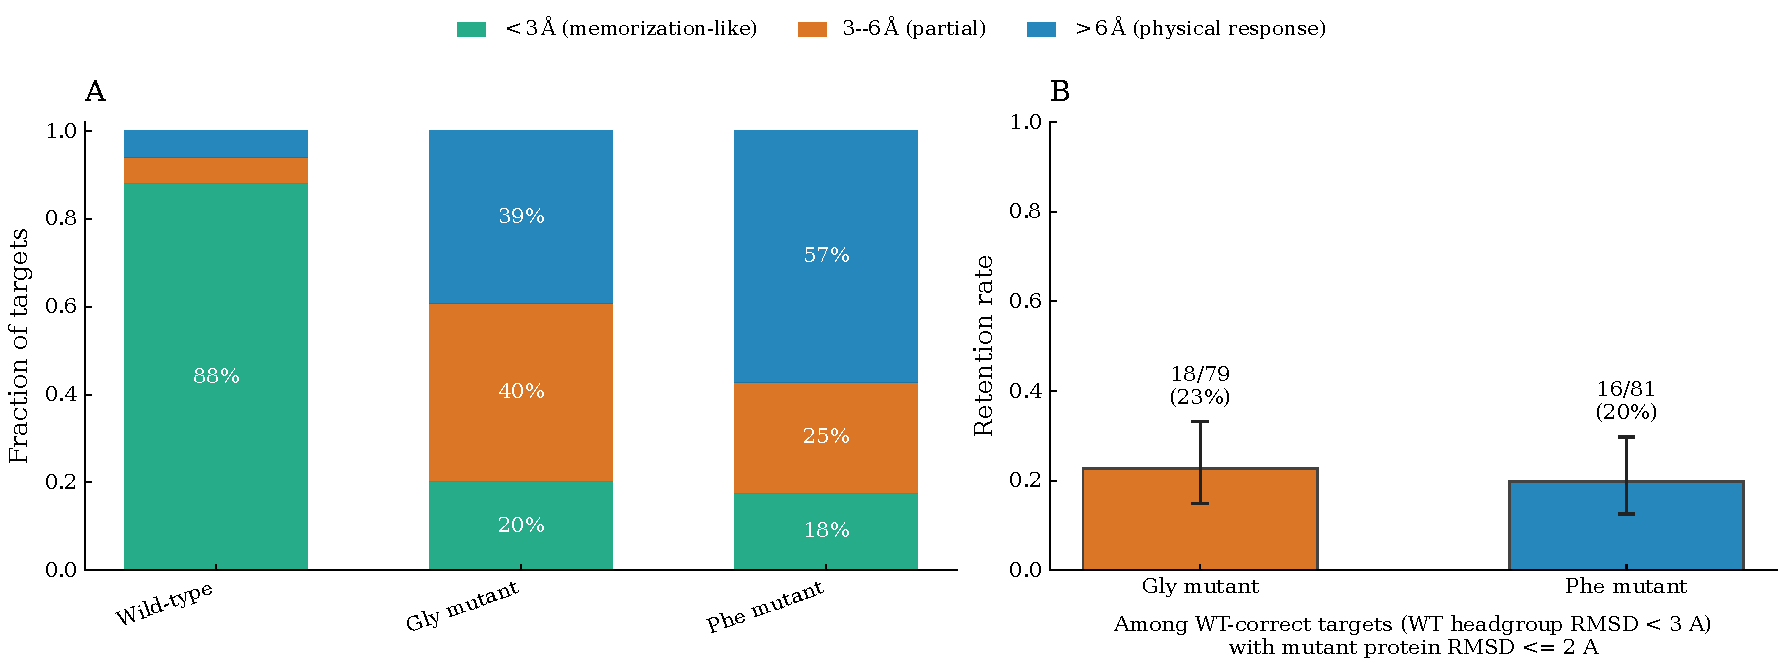
\includegraphics[width=\columnwidth]{fig_adversarial_mutagenesis_prot2A.pdf}
\caption{Adversarial binding-site mutagenesis results. (A) Outcome categories based on headgroup RMSD: strong memorization-like ($<$\SI{3}{\angstrom}), partial response (\SIrange{3}{6}{\angstrom}), or physical response ($>$\SI{6}{\angstrom}). Upon mutation, the fraction with accurate headgroup placement drops from 88\% to $\sim$20\% among fold-preserving mutants (protein RMSD $\leq$ \SI{2.0}{\angstrom}). (B) Retention analysis: among wild-type-correct targets that also satisfy the fold filter (79 Gly; 81 Phe), only 23\% (Gly) and 20\% (Phe) remain below \SI{3}{\angstrom} after mutation. Error bars show Wilson 95\% confidence intervals.}
\label{fig:adversarial}
\end{figure}
\FloatBarrier

\section{Discussion}

This benchmark shows a clear separation between AI-based complex prediction and classical docking baselines in a lipid re-docking setting.
Boltz-2 consistently produces lower ligand and headgroup RMSD and more faithfully recovers native headgroup contacts, indicating that its advantage is not limited to a single metric but reflects a more coherent pose.

The sampling-versus-ranking analysis clarifies why docking underperforms here.
In this benchmark, Vina often generates a near-native pose within its top-20 candidates, but its scoring function struggles to rank it first.
GNINA improves ranking and also shifts the best-of-20 distribution toward lower RMSD, suggesting that its scoring and local optimization pipeline yields a better candidate set, yet the gap to Boltz-2 remains substantial.
Together, these results indicate that better scoring is helpful but not sufficient on its own; capturing the coupled protein--ligand geometry (including induced fit and headgroup-specific interactions) is a key determinant of success for lipid docking.

The adversarial mutagenesis experiment provides evidence that Boltz-2's lipid placement is chemistry-dependent rather than purely memorization-driven.
When binding-site residues are mutated to glycine or phenylalanine, 75--80\% of previously accurate predictions degrade substantially, with headgroup RMSD shifting from sub-\SI{3}{\angstrom} to $>$\SI{5}{\angstrom} on average.
The phenylalanine sweep produces larger displacements than the glycine sweep, consistent with steric blockage being more disruptive than simple side-chain removal.
This sensitivity to local chemistry suggests that Boltz-2 has learned aspects of protein--lipid interaction physics, not merely where lipids ``typically sit'' in familiar protein folds.
However, the $\sim$20\% of targets that retain accurate predictions despite binding-site disruption warrant further investigation; our resistant-case analysis indicates that these are enriched for backbone-mediated headgroup contacts, supporting a backbone-dominated interaction geometry as one plausible explanation.

The headgroup interaction metrics reinforce the biological relevance of these differences.
Methods that place the headgroup accurately are also the ones that best recapitulate the protein's headgroup contact environment, supporting headgroup placement as an informative proxy for functional correctness in lipid docking.
This motivates evaluating lipid docking with interaction-based metrics alongside RMSD, rather than relying solely on tail-heavy geometric measures.

Finally, the results highlight a practical implication: in workflows where only a single ranked pose is used, ranking quality is as important as sampling.
GNINA narrows that gap but does not eliminate it, whereas Boltz-2 performs well without reliance on multi-pose reranking.
For lipid systems where headgroup chemistry and local protein interactions dominate specificity, jointly generated protein--ligand models performed especially well in this benchmark.

\subsection{Limitations}

Several important limitations should be noted.

\begin{enumerate}
    \item \textbf{Re-docking versus prospective prediction.} The docking baselines (Vina/GNINA) are evaluated in a re-docking benchmark where ligands are docked back into their cognate experimental receptors. The structures used are likely present in Boltz-2's training data. While the adversarial mutagenesis experiment provides evidence against pure memorization by showing that predictions depend on binding-site chemistry, it does not fully substitute for prospective evaluation on structures solved after Boltz-2's training cutoff, which would provide stronger evidence of generalization to novel targets.

    \item \textbf{Comparison constraints.} Boltz-2 can model protein flexibility implicitly, while Vina and GNINA use a rigid receptor. Additionally, Vina/GNINA require a user-defined search box, whereas Boltz-2 predicts the binding site de novo. A more controlled comparison might use flexible receptor docking or provide Vina/GNINA with ensemble receptor structures.

    \item \textbf{Scope of targets.} Our benchmark is restricted to single-chain proteins with single lipid ligands. Many biologically important lipid--protein interactions involve oligomeric proteins or multiple cooperative lipid binding events, which we did not evaluate; extending the benchmark to dimeric or higher-order assemblies remains future work rather than a small add-on to the present study.

	    \item \textbf{Scope of methods.} We evaluated Boltz-2, Vina, and GNINA. We prioritized methods that could be run reproducibly across the full benchmark in a local, scriptable workflow. AlphaFold3 was not included because the public AlphaFold Server supports only a narrow ligand whitelist that covers a minority of benchmark lipids, while a benchmark-wide local AF3 comparison would have required separate weight approval and substantial new infrastructure and integration work.

	\end{enumerate}

\section{Conclusion}

We present a benchmark comparing AI-based complex prediction (Boltz-2) with physics-based docking (AutoDock Vina) on 100 curated lipid--protein complexes, with GNINA CNN rescoring as an intermediate baseline.
Boltz-2 substantially outperforms Vina in both geometric accuracy and interaction fidelity on this benchmark, while GNINA improves Vina's top-1 ranking and headgroup placement but remains below Boltz-2.
Adversarial mutagenesis experiments demonstrate that Boltz-2's lipid placement depends on binding-site chemistry: mutating binding-site residues to glycine or phenylalanine causes 75--80\% of accurate predictions to degrade, providing evidence against pure memorization of training poses.
A minority of targets ($\sim$20\%) retain accurate predictions despite binding-site disruption, warranting further investigation into whether these represent backbone-dominated interactions or residual memorization.
Future work should evaluate performance on prospectively solved structures to more directly assess generalization.
The benchmark dataset, analysis code, manuscript source, and archived benchmark-result bundle are publicly available to facilitate further method development.

	\section*{Data and Code Availability}
	
	The benchmark dataset, analysis code, manuscript source, and tracked benchmark-result archive are available at \url{https://github.com/jacksonstempel/lipid_docking_benchmark}.
	The curated benchmark entry list is provided in \texttt{structures/benchmark\_entries.csv}, and the archived result tables used to reproduce the manuscript analyses are provided under \texttt{data/reproducibility/}.

\begin{suppinfo}
Benchmark composition by coarse lipid class; robustness checks for Vina exhaustiveness 256 and a higher-sampling Boltz-2 rerun; torsion-stratified docking performance; and a condensed summary of the 10 worst Boltz-2 failures (PDF).
\end{suppinfo}

\section*{Author Information}

\subsection*{Corresponding Author}

* E-mail: \href{mailto:msmit316@utk.edu}{msmit316@utk.edu}

\subsection*{Author Contributions}

J.S. designed the study, implemented the benchmark pipeline, performed the analyses, interpreted the results, and wrote the manuscript. M.S. proposed the original benchmarking idea and provided comments on the manuscript draft.

\subsection*{Notes}

The authors declare no competing interests.

\section*{Acknowledgments}

Computations were performed in part using the University of Tennessee Advanced Computing Facility (ISAAC).
Portions of the benchmark, visualization, and plotting code were developed with assistance from multiple OpenAI models, primarily GPT-5.4, via OpenAI Codex CLI.

\bibliography{references}

\begin{tocentry}
\centering
\vspace*{\fill}
\makebox[\linewidth][c]{%
  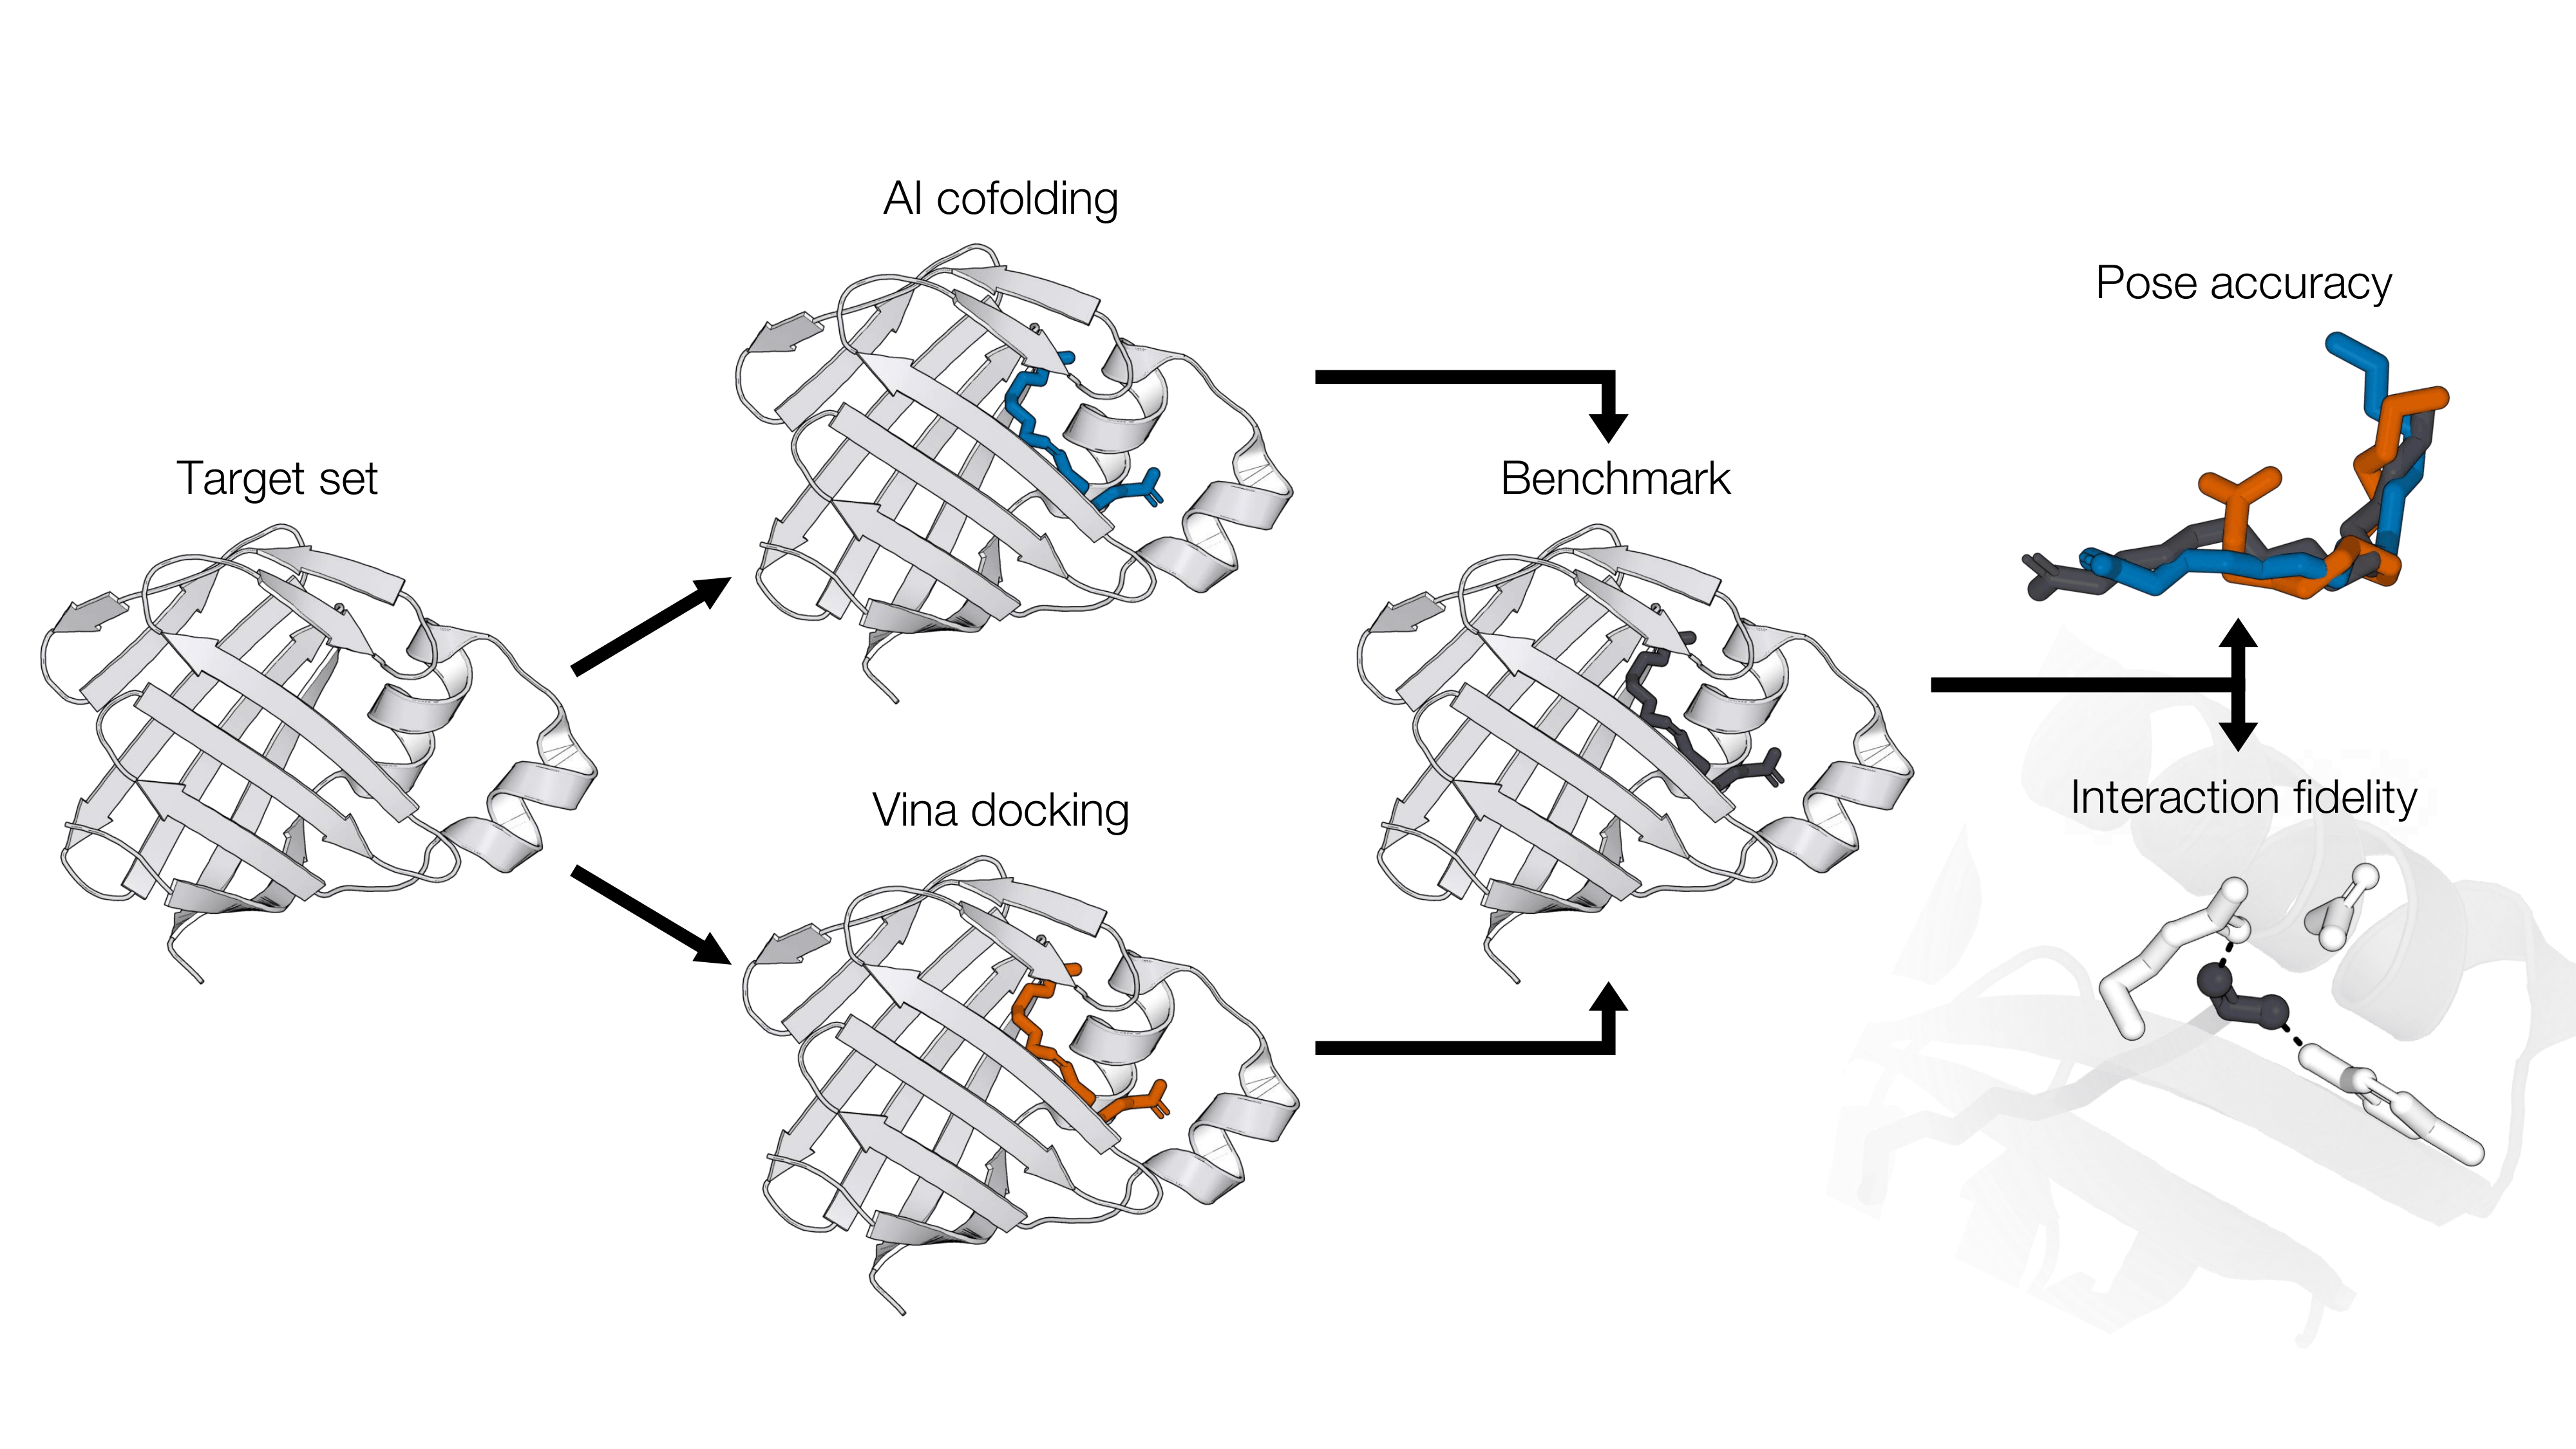
\includegraphics[height=1.55in,keepaspectratio]{toc_graphic.png}%
}
\vspace*{\fill}
\end{tocentry}

\end{document}
